\documentclass{article}
\usepackage[T1]{fontenc}
\usepackage[utf8]{inputenc}
\usepackage[portuguese]{babel}

\title{Lista 4 \\
\large Introdução à Análise Numérica \\
Solução numérica de EDOs}
\author{Lucas Emanuel Resck Domingues}
\date{\today}

\usepackage{natbib}
\usepackage{graphicx}
\usepackage{amsmath}
\usepackage{listings}
\usepackage{multirow}
\usepackage{hyperref}
\usepackage{amsfonts}

% \lstset{columns=fullflexible}

% Hyperlinks
\usepackage{hyperref}
\hypersetup{
    colorlinks=true,
    allcolors=,  % Nothing change colors
    urlcolor=blue  % URL changes color
}

\begin{document}

    \maketitle

    \begin{enumerate}
        \item[4.]
            \begin{enumerate}
                \item A função que constrói uma aproximação
                    da solução utilizando do método Forward
                    Euler foi implementada e pode ser vista
                    no Apêndice \ref{appendix:forward_euler}.

                    O intervalo de integração é particionado
                    em $N$ intervalos de comprimento igual a $h$,
                    e o método é calculado em cada ponto da partição
                    utilizando o método Forward Euler. Ao final,
                    um gráfico do valor exato e do valor aproximado
                    da função no intervalo especificado é exibido.

                    O cálculo do valor exato é obtido resolvendo
                    a EDO de forma analítica: podemos ver que a solução
                    será a exponencial de uma matriz, que pode ser
                    facilmente calculada com o uso da diagonalização.
                    De forma bastante resumida, se $x_0 = \{c_1, c_2\}$
                    e $A$ é tal que $x'(t) = A x(t)$, então

                    \begin{align*}
                        x(t) &= e^{At} x(0) \\
                        &= Pe^{Dt}P^{-1} x(0) \\
                        &= \begin{pmatrix}
                            c_1 e^{-1000*t} + \dfrac{c_2}{1000}\left(e^{-t/10} - e^{-1000*t}\right) \\[6pt]
                            c_2 e{-t/10}
                        \end{pmatrix}
                    \end{align*}

                \item As Figuras \ref{fig:forward_1},
                    \ref{fig:forward_2} e \ref{fig:forward_3}
                    exibem os resultados da aproximação para diferentes
                    valores de $h$, com intervalo de integração $[0, 1]$
                    e condição inicial $x(0) = \{1, 1\}$. Nas Figuras,
                    também vamos os erros na norma infinito, entre
                    aproximação e valor exato, além de uma comparação
                    no gráfico. Observamos que a solução para a segunda
                    coordenada, $x_2$, sempre fica boa, enquanto a solução
                    para $x_1$ só fica boa para $h < 0.002$.
                
                    \begin{figure}[!h]
                        \centering
                        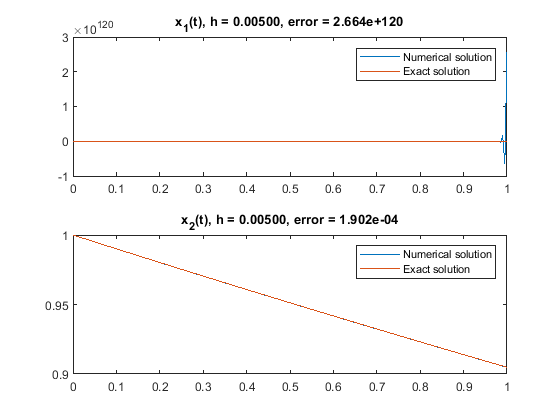
\includegraphics[width=0.8\textwidth]{images/forward_1.png}
                        \caption{Aproximação pelo método Forward Euler (em azul) e
                        solução exata (em laranja), para $h = 0.005$,
                        no intervalo $[0, 1]$, com $x(0) = \{1, 1\}$.
                        O erro calculado é a norma infinito entre as
                        soluções.}
                        \label{fig:forward_1}
                    \end{figure}
                    
                    \begin{figure}[!h]
                        \centering
                        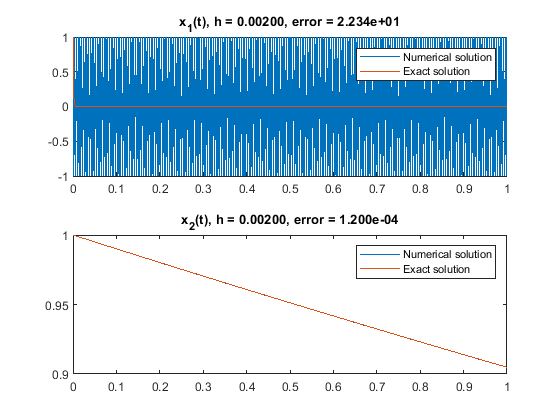
\includegraphics[width=0.8\textwidth]{images/forward_2.png}
                        \caption{Aproximação pelo método Forward Euler (em azul) e
                        solução exata (em laranja), para $h = 0.002$,
                        no intervalo $[0, 1]$, com $x(0) = \{1, 1\}$.}
                        \label{fig:forward_2}
                    \end{figure}
                    
                    \begin{figure}[!h]
                        \centering
                        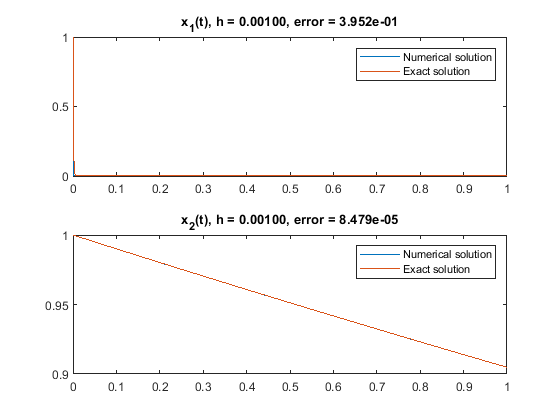
\includegraphics[width=0.8\textwidth]{images/forward_3.png}
                        \caption{Aproximação pelo método Forward Euler (em azul) e
                        solução exata (em laranja), para $h = 0.001$,
                        no intervalo $[0, 1]$, com $x(0) = \{1, 1\}$.}
                        \label{fig:forward_3}
                    \end{figure}

                    \clearpage

                    No nosso problema, temos $x' = Ax$, com $\text{Re}(\lambda) < 0$,
                    sendo $\lambda$ autovalor de $A$. De fato,
                    $\lambda_1 = -1000 < 0, \lambda_2 = -1/10 < 0$.
                    Sabemos que o domínio de estabilidade do método
                    Forward Euler é dado por
                    $\{z \in \mathbb{C} : |r(z)| = |1 + z| < 1\}$. Para que o método
                    numérico reproduza a dinâmica da solução, devemos ter

                    \begin{align*}
                        &|r(\lambda h)| < 1 \\
                        \Rightarrow &|1 + \lambda h| < 1 \\
                        \Rightarrow &\begin{cases}
                            |1 -1000 h| < 1 \\
                            \left|1 - \dfrac{1}{10} h\right| < 1 \\
                        \end{cases} \\
                        \Rightarrow &0 < h < 0.002
                    \end{align*}
                    
                    Conclusão: o método só reproduz a dinâmica da solução
                    exata quando $h < 0.002$, o que pode ser verificado nos
                    resultados numéricos.

                \item O método Backward Euler foi implementado e seu código
                    pode ser visualizado no Apêndice \ref{appendix:backward_euler}.
                    
                    O algoritmo é muito semelhante àquele do método Forward Euler.
                    A principal diferença é o cálculo de $x_{k+1}$ a partir de
                    $x_k$. No método Foward Euler, isso é direto. Porém, agora,
                    com o Backward Euler, temos:

                    \begin{align*}
                        &x_{k+1} = x_k + f(t_{k+1}, x_{k+1}) h \\
                        \Rightarrow &x_{k+1} = x_k + Ax_{k+1} h \\
                        \Rightarrow &(I - Ah)x_{k+1} = x_k \\
                        \Rightarrow &M x_{k+1} = x_k \\
                    \end{align*}

                    Isso é um sistema linear $2\times2$ a ser resolvido. Acredite, a matriz
                    é diagonalmente dominante, e isso é fácil de ser verificado.
                    O algoritmo do Apêndice \ref{appendix:backward_euler} implementa
                    o método de Seidel para sua resolução.

                    As Figuras \ref{fig:backward_1}, \ref{fig:backward_2},
                    \ref{fig:backward_3} e \ref{fig:backward_4}
                    exibem os resultados da aproximação para diferentes
                    valores de $h$, com intervalo de integração $[0, 1]$
                    e condição inicial $x(0) = \{1, 1\}$. Nas Figuras,
                    também vamos os erros na norma infinito, entre
                    aproximação e valor exato, além de uma comparação
                    no gráfico. Observamos que a solução para as duas
                    coordenadas, $x_1$ e $x_2$, ficam boas, para qualquer
                    valor de $h$.
                
                    \begin{figure}[!h]
                        \centering
                        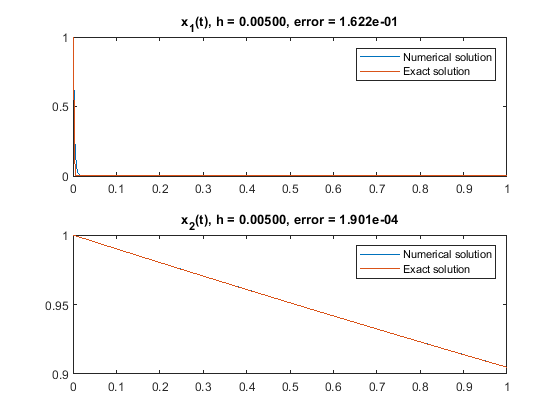
\includegraphics[width=0.8\textwidth]{images/backward_1.png}
                        \caption{Aproximação pelo método Backward Euler (em azul) e
                        solução exata (em laranja), para $h = 0.005$.}
                        \label{fig:backward_1}
                    \end{figure}
                
                    \begin{figure}[!h]
                        \centering
                        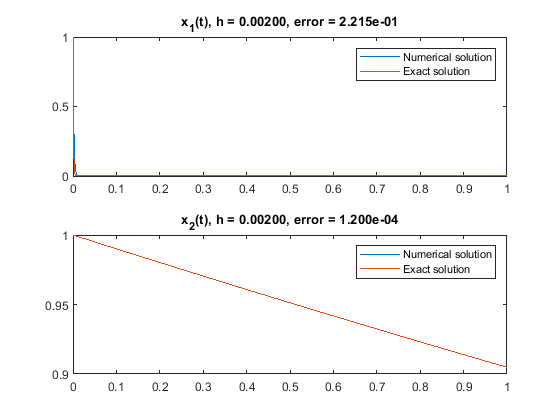
\includegraphics[width=0.8\textwidth]{images/backward_2.png}
                        \caption{Aproximação pelo método Backward Euler (em azul) e
                        solução exata (em laranja), para $h = 0.002$.}
                        \label{fig:backward_2}
                    \end{figure}
                
                    \begin{figure}[!h]
                        \centering
                        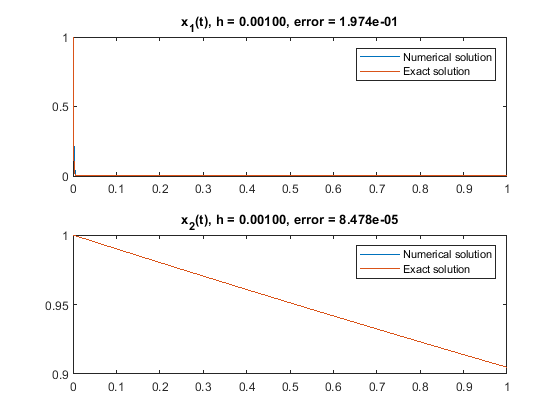
\includegraphics[width=0.8\textwidth]{images/backward_3.png}
                        \caption{Aproximação pelo método Backward Euler (em azul) e
                        solução exata (em laranja), para $h = 0.001$.}
                        \label{fig:backward_3}
                    \end{figure}
                
                    \begin{figure}[!h]
                        \centering
                        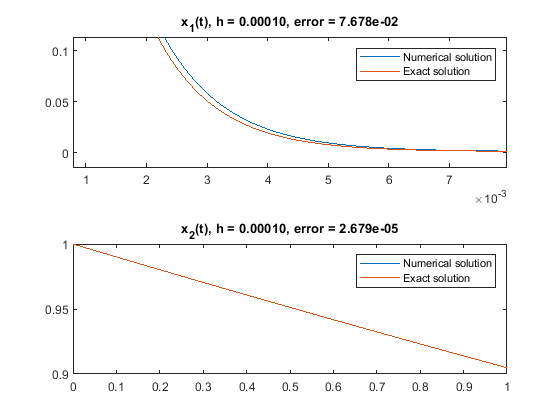
\includegraphics[width=0.8\textwidth]{images/backward_4.png}
                        \caption{Aproximação pelo método Backward Euler (em azul) e
                        solução exata (em laranja), para $h = 0.0001$.}
                        \label{fig:backward_4}
                    \end{figure}

                    \clearpage

                    Verificamos que o desempenho do método
                    Backward Euler é bem melhor. Isso se dá,
                    entre outras coisas, pelo fato de que
                    o domínio de estabilidade desse método é
                    (infinitamente) melhor. Ele é:

                    \begin{align*}
                        &|r(\lambda h)| < 1 \\
                        \Rightarrow &\left|\dfrac{1}{1 - \lambda h}\right| < 1 \\
                        \Rightarrow &\begin{cases}
                            \left|\dfrac{1}{1 + 1000 h}\right| < 1 \\
                            \left|\dfrac{1}{1 + \frac{1}{10} h}\right| < 1 \\
                        \end{cases} \\
                        \Rightarrow & h > 0
                    \end{align*}

                    Ou seja, qualquer que seja $h$, temos um método A-estável.

            \end{enumerate}

            \pagebreak

            \item[6.]
                \begin{enumerate}
                    \item A função que implementa o método RK4 clássico
                        para aproximar a solução da EDO pode ser conferida
                        no Apêndice \ref{appendix:runge_kutta}.

                        O método de Runge-Kutta foi implementado de forma
                        semelhante aos método anteriores, no que diz respeito
                        ao cálculo do número de iterações e da atualização
                        da solução numérica. A diferença é a função que é 
                        utilizada para a aproximação numérica, própria deste
                        método.

                        A função também compara as soluções exata e aproximada
                        em um gráfico, além de exibir o erro (na norma infinito)
                        entre as soluções. O resultado da execução da função para
                        $h = 0.5$, $T = 20$, $k = 0.01$, $a = 70$, $b = 50$ pode ser
                        conferido na Figura \ref{fig:rk_1}.
                
                        \begin{figure}[!h]
                            \centering
                            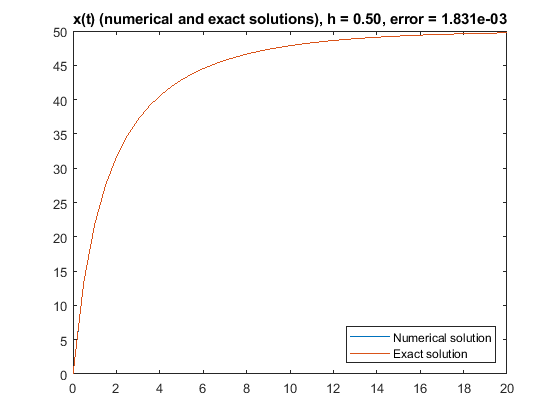
\includegraphics[width=0.8\textwidth]{images/rk_1.png}
                            \caption{Soluções exata e numérica (RK4 clássico)
                            da função $x$.}
                            \label{fig:rk_1}
                        \end{figure}

                    \item O programa foi testado para diferentes valores de $T$,
                        e as comparações entre os valores exato e numérico
                        podem ser conferidas nas Figuras
                        \ref{fig:rk_2}, \ref{fig:rk_3} e \ref{fig:rk_4}.
                
                        \begin{figure}[!h]
                            \centering
                            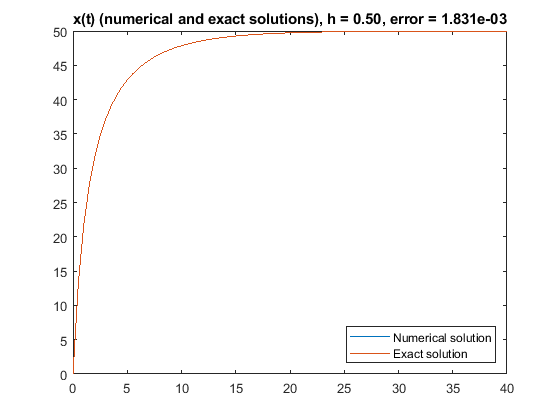
\includegraphics[width=0.8\textwidth]{images/rk_2.png}
                            \caption{Soluções exata e numérica (RK4 clássico)
                            da função $x$.}
                            \label{fig:rk_2}
                        \end{figure}
                
                        \begin{figure}[!h]
                            \centering
                            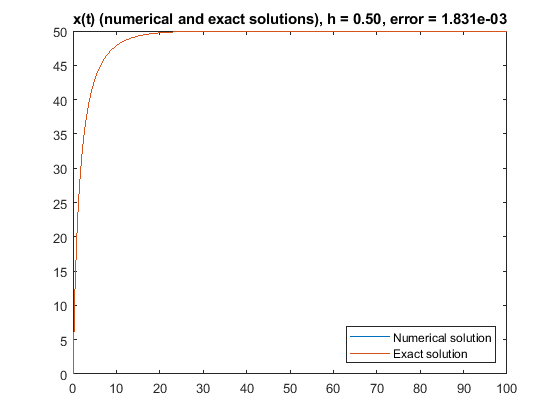
\includegraphics[width=0.8\textwidth]{images/rk_3.png}
                            \caption{Soluções exata e numérica (RK4 clássico)
                            da função $x$.}
                            \label{fig:rk_3}
                        \end{figure}
                
                        \begin{figure}[!h]
                            \centering
                            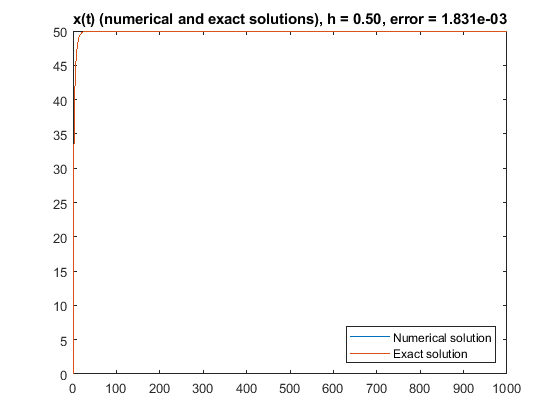
\includegraphics[width=0.8\textwidth]{images/rk_4.png}
                            \caption{Soluções exata e numérica (RK4 clássico)
                            da função $x$.}
                            \label{fig:rk_4}
                        \end{figure}

                        \clearpage

                        Observamos que não foi necessário ajustar o parâmetro
                        $h$ para que houvesse convergência, deixando-o como
                        $h = 0.5$ anteriormente dado. Vemos que a solução
                        numérica aproxima muito bem a solução real, em todos
                        esses casos.

                    \item Observamos através dos gráficos que o método RK4 reproduz
                        o comportamento assintótico da solução exata. Portanto,
                        concluímos que, sim, existe valor fixo de $h$ que satisfaz
                        isso. No nosso caso, bastou $h = 0.5$.
                \end{enumerate} 
    \end{enumerate}

    \clearpage

    \appendix

    \section{Forward Euler}
        \label{appendix:forward_euler}

        Código em Matlab para o exercício 4. Também pode ser conferido
        \href{https://github.com/lucasresck/introduction-to-numerical-analysis/blob/master/list_4/forward_euler_4.m}{neste link}.

        \begin{lstlisting}[language=Matlab]
function [t, x] = forward_euler_4(h, t_0, T, x_0)
    % Approximate the solution with Forward Euler method.
    % Examples:
        % [t, x] = forward_euler_4(0.0001, 0, 1, [1;1]);
        % [t, x] = forward_euler_4(0.01, 0, 1, [1;1]);
    x = [x_0];
    t = [t_0];
    N = floor((T - t_0)/h);
    for k = 1:N
        x_k_old = x(:, end);
        t_k_old = t(end);
        x_k = x_k_old + f(x_k_old)*h;
        x = [x, x_k];
        t_k = t_0 + k*h;
        t = [t, t_k];
    end
    plot_solutions(t, x, x_0, h)
end

function result = f(x)
    % Calculate f.
    A = [-1000, 1; 0, -1/10];
    result = A*x;
end

function plot_solutions(t, x, x_0, h)
    % Plot the exact and numerical solutions.
    y1 = x(1, :);
    y2 = x(2, :);
    y = exact_x(t, x_0);
    tiledlayout(2,1)
    
    % Plot the first coordinate
    nexttile
    plot(t, y1)
    hold on
    plot(t, y(1, :))
    hold off
    legend({'Numerical solution', 'Exact solution'}, ...
    'Location', 'northeast')
    error_1 = (norm(y1 - y(1, :)));
    title(sprintf('x_1(t), h = %0.5f, error = %0.3e', h, error_1))

    % Plot the second coordinate
    nexttile
    plot(t,y2)
    hold on
    plot(t, y(2, :))
    hold off
    legend({'Numerical solution', 'Exact solution'}, ...
    'Location', 'northeast')
    error_2 = (norm(y2 - y(2, :)));
    title(sprintf('x_2(t), h = %0.5f, error = %0.3e', h, error_2))
end

function x = exact_x(t, x_0)
    % Calculate the exact value of x(t).
    c_1 = x_0(1);
    c_2 = x_0(2);
    x_1 = c_1*exp(-1000*t) + c_2*(exp(-t/10)/1000 - exp(-1000*t)/1000);
    x_2 = c_2*exp(-t/10);
    x = [x_1; x_2];
end
        \end{lstlisting}

    \section{Backward Euler}
        \label{appendix:backward_euler}

        Código em Matlab para o exercício 4. Também pode ser conferido
        \href{https://github.com/lucasresck/introduction-to-numerical-analysis/blob/master/list_4/backward_euler_4.m}{neste link}.

        \begin{lstlisting}[language=Matlab]
function [t, x] = backward_euler_4(h, t_0, T, x_0)
    % Approximate the solution with Backward Euler method.
    % Examples:
        % [t, x] = backward_euler_4(0.0001, 0, 1, [1;1]);
        % [t, x] = backward_euler_4(0.01, 0, 1, [1;1]);
    x = [x_0];
    t = [t_0];
    N = floor((T - t_0)/h);
    for k = 1:N
        x_k_old = x(:, end);
        t_k_old = t(end);
        x_k = seidel(x_k_old, 10^-3, h);
        x = [x, x_k];
        t_k = t_0 + k*h;
        t = [t, t_k];
    end
    plot_solutions(t, x, x_0, h)
end

function x = seidel(b, eps, h)
    % Solve linear system with Seidel method.
    x = zeros(2, 1);
    err = 1 + eps;
    x_old = x;
    C = [0, h/(1+1000*h); 0, 0];
    d = b ./ [1+1000*h;1+1/10*h];
    while err > eps
        x = C*x_old + d;
        err = norm(x - x_old, 'inf')/norm(x_old, 'inf');
        x_old = x;
    end
end

function plot_solutions(t, x, x_0, h)
    % Plot the exact and numerical solutions.
    y1 = x(1, :);
    y2 = x(2, :);
    y = exact_x(t, x_0);
    tiledlayout(2,1)
    
    % Plot the first coordinate
    nexttile
    plot(t, y1)
    hold on
    plot(t, y(1, :))
    hold off
    legend({'Numerical solution', 'Exact solution'}, ...
    'Location', 'northeast')
    error_1 = (norm(y1 - y(1, :)));
    title(sprintf('x_1(t), h = %0.5f, error = %0.3e', h, error_1))

    % Plot the second coordinate
    nexttile
    plot(t,y2)
    hold on
    plot(t, y(2, :))
    hold off
    legend({'Numerical solution', 'Exact solution'}, ...
    'Location', 'northeast')
    error_2 = (norm(y2 - y(2, :)));
    title(sprintf('x_2(t), h = %0.5f, error = %0.3e', h, error_2))
end

function x = exact_x(t, x_0)
    % Calculate the exact value of x(t).
    c_1 = x_0(1);
    c_2 = x_0(2);
    x_1 = c_1*exp(-1000*t) + c_2*(exp(-t/10)/1000 - exp(-1000*t)/1000);
    x_2 = c_2*exp(-t/10);
    x = [x_1; x_2];
end
        \end{lstlisting}

    \section{Runge-Kutta 4 clássico}
        \label{appendix:runge_kutta}

        Código em Matlab para o exercício 6. Também pode ser conferido
        \href{https://github.com/lucasresck/introduction-to-numerical-analysis/blob/master/list_4/rk4_6.m}{neste link}.

        \begin{lstlisting}[language=Matlab]
function x = rk4_6(h, T, k, a, b)
    % Calculate the Runge-Kutta fourth-order method
    % Example:
        % x = rk4_6(0.5, 20, 0.01, 70, 50);
    x_0 = 0;
    t_0 = 0;
    x = [x_0];
    t = [t_0];
    N = floor((T - 0)/h);
    for i = 1:N
        x_i_old = x(end);
        k_1 = f(x_i_old, k, a, b);
        k_2 = f(x_i_old + h/2*k_1, k, a, b);
        k_3 = f(x_i_old + h/2*k_2, k, a, b);
        k_4 = f(x_i_old + h*k_3, k, a, b);
        phi = 1/6*(k_1 + 2*k_2 + 2*k_3 + k_4);
        x_i = x_i_old + h*phi;
        x = [x, x_i];
        t_i = t_0 + i*h;
        t = [t, t_i];
    end
    plot_solutions(t, x, h);
end

function y = f(x, k, a, b)
    % Calculate f.
    y = k*(a - x)*(b - x);
end

function plot_solutions(t, x, h)
    % Plot the exact and numerical solutions.
    plot(t, x);
    hold on;
    plot(t, exact_x(t));
    hold off;
    error = norm(x - exact_x(t), 'inf');
    title(...
        sprintf(...
        'x(t) (numerical and exact solutions), h = %0.2f, error = %0.3e', ...
        h, error))
    legend({'Numerical solution', 'Exact solution'}, ...
    'Location', 'southeast')
end

function x = exact_x(t)
    % Calculate the exact value of x(t).
    x = 350*(1 - exp(-0.2*t))./(7 - 5*exp(-0.2*t));
end
        \end{lstlisting}

\end{document}
